\documentclass[crop,tikz]{standalone}
\usepackage{chemfig}

\definecolor{spectrumcolor}{HTML}{23373B}

\begin{document}

\begin{tikzpicture}
%\draw[help lines] (0,0) grid (10,10);
\node (a) at (0,0) [anchor=south west]
{
    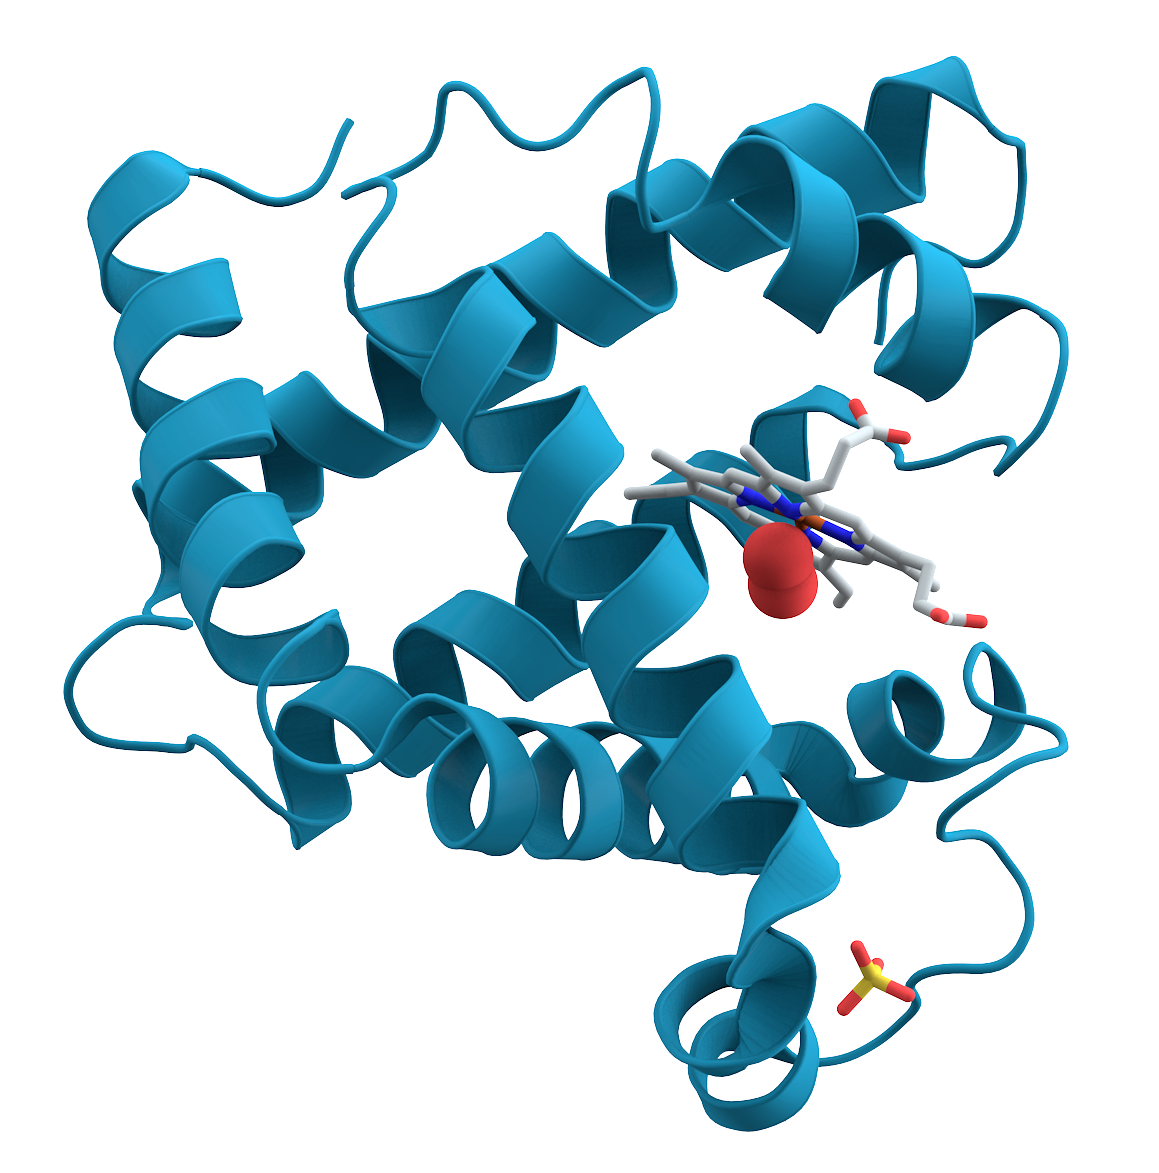
\includegraphics[width=0.75\textwidth]{myoglobin.png}
};
\node (b) at (a.east) [anchor=west, shift={(3,0)}]
{
    \begin{tikzpicture}
\definecolor{spectrumcolor}{HTML}{23373B}

%\draw[help lines, color=gray, dashed] (0,0) grid (10,10);

\tikzstyle{axis}=[line width=4pt, color=spectrumcolor]
\tikzstyle{peak}=[line width=4pt, color=spectrumcolor]

% x-axis
\draw[axis] (0,0) -- (10,0);
% peaks
\draw[peak] (1.5,0) -- (1.5,3);
\draw[peak] (2,0) -- (2,5);
\draw[peak] (3,0) -- (3,1);
\draw[peak] (5,0) -- (5,4);
\draw[peak] (7,0) -- (7,7);
\draw[peak] (7.5,0) -- (7.5,2);
\draw[peak] (8,0) -- (8,4);

\end{tikzpicture}

};
\draw [->, line width=2pt, color=spectrumcolor] (a)--(b);
\end{tikzpicture}
\end{document}
